\section{Design and Implementation}

The methodology consist of three parts, where each part builds upon the results from the previous one.
Initially the test data is created, which will be used for all evaluations.
Once the data is available, we evaluate HDBSCAN and determine the settings,
which lead to optimal results regarding our specific use case.
The final part applies the results obtained from the previous evaluation in an online setting.

\subsection{Data flow}
% Todo: Add a box diagram of the data flow
% E.g. News article -> Text preprocessing -> Clustering -> Output

\begin{tikzpicture}[
    squarednode/.style={rectangle, align=center, draw=black!60, very thick, minimum size=5mm},
    ]

    %Nodes
    \node[squarednode] (newsarticle)                                {Collection of\\ news articles};
    \node[squarednode] (preprocessing)  [right=of newsarticle]      {Text preprocessing};
    \node[squarednode] (vectorization)  [right=of preprocessing]    {Vectorization};
    \node[squarednode] (clustering)     [right=of vectorization]    {Clustering};
    \node[squarednode] (result)         [right=of clustering]       {Result};
     
    %Lines
    \draw[->] (newsarticle.east) -- (preprocessing.west);
    \draw[->] (preprocessing.east) -- (vectorization.west);
    \draw[->] (vectorization.east) -- (clustering.west);
    \draw[->] (clustering.east) -- (result.west);

\end{tikzpicture}
    
TODO describe

\subsection{Data Set}
\label{subsec:4a_data_set}

Before any clustering method can be implemented or evaluated,
it is important to rely on the right data set for training and evaluation.

\subsubsection{Data Set Candidates}
\label{subsubsec:4a_data_set_candidates}

As our goal is to detect events in data streams, we have evaluated different data sets and
their possibilities to extract events from their data themselves.

\begin{table}[h]
    \centering
    \begin{tabular}{|l|r|l|}
    \hline
    \textbf{Data set} & \textbf{Number of rows} & \textbf{Description} \\ \hline
    GDELT 2.0 & 575,000,000+ & Print and web news from around the world. \\ \hline
    ChallengeNetwork & 4,449,294 & Network packages including anomalies. \\ \hline
    One Million Posts Corpus & 1,011,773 & User comments to news articles. \\ \hline
    Online Retail Data Set & 541,909 & Customer retail purchases of one year. \\ \hline
    News Aggregator Dataset & 422,937 & Clustered news articles. \\ \hline
    Dodgers Loop Sensor Data Set & 50,400 & Number of cars driven through a ramp. \\ \hline
    10k German News Articles & 10,273 & German news articles. \\ \hline
    \end{tabular}
    \caption{Evaluated data set candidates ordered by data set size.}
    \label{tab:data_set_candidates}
\end{table}

We could extract events from all data sets mentioned in \tabref{tab:data_set_candidates}.\\
The extracted events could be as follows:

\begin{itemize}
    \item Network packages
        \begin{itemize}
            \item Cyber attacks depending on suspicious packets.
        \end{itemize}
    \item User comments
        \begin{itemize}
            \item Change of public opinion during time.
        \end{itemize}
    \item Retail purchases
        \begin{itemize}
            \item Change of purchasing behavior based on product choices.
        \end{itemize}
    \item Traffic
        \begin{itemize}
            \item Traffic changes due to baseball games.
        \end{itemize}
    \item News articles
        \begin{itemize}
            \item Development of a certain news story.
        \end{itemize}
\end{itemize}

However, from above data sets only two contained prelabeled events:

\begin{enumerate}
    \item Dodgers Loop Sensor Data Set
        \begin{itemize}
            \item 81 labeled events. % Todo: x events in y clusters
        \end{itemize}
    \item News Aggregator Dataset
        \begin{itemize}
            \item 422,937 labeled events. % Todo: x events in y clusters
        \end{itemize}
\end{enumerate}

As we did not want to lose too much time in manually clustering data,
we have decided to go with one of these two.
Regarding our two options, our choice was simple:\\
We went for the \textbf{The News Aggregator Dataset} since it not only provided more data,
but our work built on the news articles use case could later be continued with real live data.
The \textbf{GDELT 2.0} data set for example, provides around 1,000 to 2,000 new news articles every 15 minutes.

\subsubsection{Data Retrieval}
\label{subsubsec:4a_data_retrieval}

Unfortunately the data set did not contain the news articles themselves but rather only the URL's to the news articles.
This was done so due to copyright restrictions on the content.
Fortunately there are web scraping tools designed to retrieve the content from news articles specifically.
We decided to use Newspaper3k\cite{newspaper3k},
a Python3 library that allows us to retrieve the text from news articles easily.

The library only requires an URL to download and extract the news article from a website, see following example:

% Todo: Hyphen gets converted inside "lstlisting".
% Copy & paste the URL from the PDF into a browser -> it won't work.
\begin{lstlisting}[language=Python, caption=Retrieve the news article from an URL., label={lst:newspaper3k_code}]
    from newspaper import Article

    url = 'http://fox13now.com/2013/12/30/new-year-new-laws-obamacare-pot-guns-and-drones/'
    article = Article(url)
    article.download()
    article.text # Contains the article's text.
\end{lstlisting}

All we had to do now is to run this code for all news articles.
To speed this process up, we have loaded the data set into a database and run 8 concurrent processes which
retrieved the news articles content from the web in different batches.

\subsubsection{Data Cleansing}
\label{subsubsec:4a_data_cleansing}

The data set contains news articles collected from March 10th to August 10th of 2014.
Five years later, many resources are not online anymore or are not accessible from Europe due to GDPR.
We have used following SQL query to filter out news articles that were most likely corrupt:

\begin{lstlisting}[language=SQL, caption=Retrieve valid news articles., label={lst:valid_news_articles_sql}]
    SELECT *
    FROM news_article
    WHERE
        newspaper_text IS NOT NULL
        AND TRIM(COALESCE(newspaper_text, '')) != ''
        AND hostname NOT IN ('newsledge.com', 'www.newsledge.com')
        AND newspaper_text NOT LIKE '%GDPR%'
        AND newspaper_text NOT LIKE '%javascript%'
        AND newspaper_text NOT LIKE '%404%'
        AND newspaper_text NOT LIKE '%cookie%'
        AND newspaper_keywords NOT LIKE '%GDPR%'
        AND newspaper_keywords NOT LIKE '%javascript%'
        AND newspaper_keywords NOT LIKE '%404%'
        AND newspaper_keywords NOT LIKE '%cookie%'
        AND title_keywords_intersection = 1
\end{lstlisting}

% Todo: Continue cleansing text.

% Todo: The first important step is to create a test data set to run the evaluations with and verify them.
% Todo: explain the source and structrue

% raw text
% with entity extraction
% word embeddings?
% Tfidf

\subsection{Clustering Evaluation}
\label{subsec:4b_clustering_evaluation}

\subsubsection{Design}
\label{subsubsec:4b_design}

The goal of the clustering evaluation is to find the optimal parameters and preprocessing methods for applying HDBSCAN in an online setting.
Therefore the clustering evaluation is designed to run HDBSCAN on our test data,
using a combination of different text processing methods, vector space models and parameters.
\textit{k}-means is used to provide a benchmark for HDBSCAN evaluation.
Once a clustering has been performed, the result is measured based on the ground truth and stored in a database for later analysis.

An important consideration is the variety of samples to use for a clustering run.
Using only a single set of samples might bias the score against this specific set of samples
and some methods might perform better or worse depending on the samples.
To introduce variability, while still retaining repeatability, an evaluation run will be repeated multiple times.
Each repetition will load a new set of sample, iterating linearly through the data set.
For example if we define the number of repetitions as two with a sample size of 1000,
the evaluation will first be done on the first 1000 samples with all possible settings
and the second run will load the next 1000 samples, thus containing sample with indices ranging from 1001 to 2000.
The reason we do not load random sets of samples is repeatability.
If we make any changes in the implementation or the scoring function,
we want to be able to compare the new results with the previous ones in a deterministic manner.

\subsubsection{Scoring Function}
\label{subsubsec:4b_scoring_function}

The scoring function is essential for measuring the result of a clustering method.
The score should reflect the quality of the individual clusters and of the clustering as a whole.
The number of existing measures for clustering is vast and can be split into two main categories.
Internal measures determine the score based on criteria derived from the data itself
and external measures depend on criteria non-existent in the data itself such as class labels.
Since the ground truth is known in our test data, we are going to apply an external measure.

Initially we used Normalized Mutual Information (NMI) as our primary scoring function.
The NMI is an entropy-based measure and tries to quantify the amount shared information between the clusterings.
The score proved to work well for our initial evaluations, but upon closer inspection certain anomalies were found.
An example is given in table \ref{tab:nmi_kmeans_example}, where \textit{k}-means achieved a rather high score,
regardless of the large difference between the true amount of clusters and the approximation using $\sqrt{n}$.
We were not able to explain this behaviour,
although there are multiple papers about the selection bias of NMI for higher numbers of clusters\cite{LEI201758}\cite{clustering_anmi}.
Other scoring functions such as V-Measure or the Adjusted Rand Index showed similar unexpected results with different clusterings.
Therefore we decided to develop our own scoring function based on the ideas of Maximum Matching\cite{data_mining}
and the Jaccard Index, which we call MP-Score.

% TODO add number of estimated clusters
\begin{table}[h]
    \centering
    \begin{tabular}{|l|l|l|l|l|}
    \hline
    \textbf{Algorithm} & \textbf{Sample Size} & \textbf{NMI}  & $\mathbf{n_{true}}$ & $\mathbf{ \mid n_{true} - n_{predicted} \mid }$ \\ \hline
    \textit{k}-means & 19255 & 0.754 & 600 & 457 \\ \hline
    HDBSCAN & 19255 & 0.742 & 600 & 2 \\ \hline
    \end{tabular}
    \caption{\textit{k}-means has a higher NMI score than HDBSCAN, while having a much larger difference in number of clusters.}
    \label{tab:nmi_kmeans_example}
\end{table}

\paragraph{Calculating the score}
The scoring function first calculates the similarity between pairs of clusters,
where each cluster belongs to a different clustering.
We use the Jaccard Index to measure the similarity, which is defined as

\begin{equation}
    \label{equ:similarity}
    \frac{|A \cap B|}{|A \cup B|}
\end{equation}

To illustrate the process we start with an example.
We use $T$ and $C$ as our clusterings, where $T$ is the ground truth and $C$ is the predicted clustering.
The clusterings are defined as follows:

\begin{gather*}
    T = \{\{1,2,3\},\{4,5,6,7\},\{8,9\}\} \\
    C = \{\{1,2\},\{3,4,5,6\},\{7\},\{8,9\}\}
\end{gather*}

We calculate the similarity as defined in Equation \eqref{equ:similarity},
for each possible pair between $T$ and $C$ starting with $t_1= \{1,2,3\}$ and $c_1 = \{1,2\}$:

\begin{align*}
    similarity(t_1,c_1) &=\frac{|t_1 \cap c_1|}{|t_1 \cup c_1|}
    = \frac{|\{1,2\}|}{|\{1,2,3\}|}
    = \frac{2}{3} = 0.667 \\
\end{align*}

After doing this for each possible pair we get the similarity matrix $A$:

\begin{gather*}
\begin{array}{rcl}
    A = & \left(\begin{array}{cccc}
        similarity(t_1,c_1) & \hdots & \hdots & similarity(t_1,c_4)\\
        \vdots & \vdots & \vdots & \vdots\\
        similarity(t_3,c_3) & \hdots & \hdots & similarity(t_3,c_4) \end{array}\right)
        = & \left(\begin{array}{cccc}
            0.667 & 0.167 & 0 & 0 \\
            0 & 0.6 & 0.25 & 0.4 \\
            0 &  0 & 0 & 1.0 \end{array}\right)
\end{array}
\end{gather*}

As a next step we have to select the most relevant similarity values from each row of the similarity matrix.

Finding relevant values in the similarity matrix is non-trivial,
since clusters do not share labels across different clusterings.
To solve this, we make two assumptions based on the principle of Maximum Matching:

\begin{enumerate}
    \item The higher the similarity between two clusters, the more likely it is, that both clusters are describing the same group of documents.
    \item Each cluster can be associated with a cluster from another clustering only once.
\end{enumerate}

Based on those assumptions we select the highest similarity value per row,
whose column is not already associated with another row.
Applying this selection function $f$ to our previously calculated similarity matrix $A$
results in the set containing the most relevant similarity values.

\begin{gather*}
    \begin{array}{rcl}
        f(A) = & \left(\begin{array}{cccc}
            \mathbf{0.667} & 0.167 & 0 & 0 \\
            0 & \mathbf{0.6} & 0.25 & 0.4 \\
            0 &  0 & 0 & \mathbf{1.0} \end{array}\right)
            = \{0.667, 0.6, 1\}
    \end{array}
\end{gather*}

As we can see, there were no collisions between columns and we simply get the highest value per row.
Consider the following example with a different similarity matrix $B$, which does contain a collision:

\begin{gather*}
    \begin{array}{rcl}
        f(B) = & \left(\begin{array}{cccc}
            \mathbf{0.75} & 0.375 & 0.427 & 0.375 \\
            0.4 & \mathbf{0.667} & 0.571 & \textcolor{red}{0.8} \\
            0.333 &  0.25 & 0.4 & \mathbf{1.0} \end{array}\right)
            = \{0.75, 0.667, 1\}
    \end{array}
\end{gather*}

The selected similarity for the second row is 0.667 instead of 0.8.
This is because the fourth column is already associated with the third row, while having an similarity greater than 0.8.
Therefore based on our assumption that clusters cannot be associated twice,
the second highest similarity is used for the second column.
In case no association could be found, the value would be set to zero.

As a third step we have to calculate the weights to be used for the weighted average.
The weight is based on the number of elements inside the cluster
and necessary to represent differences in predicted and true number of clusters in the final score.
It is defined as follows:

\begin{equation}
    \label{equ:weight}
        w_{ij} = \frac{|t_i| + |c_j|}{|T|+|C|} \\
\end{equation}

where $T$ is the ground truth with $t_i \in T$ and $C$ the predicted clustering with  $c_j \in C$.
Therefore the weight for a pairing $t_ic_j$ includes both the size of the true cluster and the size of the predicted cluster.
The reason both sizes are used, is that we want to reflect the difference between the number of predicted clusters and the ground truth.
Using only the true number of elements as the weight, would affect the score if $|C| < |T|$, but not $|C| > |T|$.
Hence the number of predicted elements has to be included into the weight.

To continue our example we have to calculate the weights based on the coordinates of the selected values from our similarity matrix $A$.
The coordinates are $(1,1), (2,2), (3,4)$.
As a result we calculate the following weights:

\begin{align*}
    w_{1,1} &= \frac{|t_1| + |c_1|}{|T|+|C|} = \frac{3 + 2}{9 + 9} = \frac{5}{18} = 0.278 \\
    w_{2,2} &= \frac{|t_2| + |c_2|}{|T|+|C|} = \frac{4 + 4}{9 + 9} = \frac{8}{18} = 0.444 \\
    w_{3,4} &= \frac{|t_3| + |c_4|}{|T|+|C|} = \frac{2 + 2}{9 + 9} = \frac{4}{18} = 0.222
\end{align*}

In the fourth and final step we calculate the weighted average

\begin{equation}
    \label{equ:weighted_average}
        \text{MP-Score} = \sum_{i=0}^{|S|} w_is_i \{w_i \in W \wedge s_i \in S\}
\end{equation}

where $S$ contains the selected values from the similarity matrix with $s_{i} \in S$ and $W$ is the set of weights with $w_i \in W$.
Using our previously selected similarity values $S = f(A) = \{0.667, 0.6, 1\}$
and the corresponding weights $W = \{0.278, 0.444, 0.222\}$,
the calculation for the final average would be done as follows:

\begin{align*}
    \text{MP-Score} = (0.278 \cdot 0.667) + (0.444 \cdot 0.6) + (0.222 \cdot 1) = \mathbf{0.674}
\end{align*}

The final score for the evaluation of the predicted cluster $C$ with the true cluster is 0.674.
The complete implementation of the scoring function can be found in the appendix as Listing \ref{lst:select_max_values}.

\paragraph{Comparison against other measures}
The test scenarios in table \ref{tab:score_scenarios} show the resulting scores of our similarity score, NMI and ARI.
The second scenario results in a ARI score of 0.308, while the NMI with 0.564 and the MP-Score with 0.637 are both higher.
Intuitively we would assume the higher score to better represent the predicted clustering,
since the number of clusters is correct and only two out of nine elements are assigned to the wrong cluster.
Scenario six shows a similar case.
Scenarios four and especially five show the previously mentioned bias of NMI with regards to higher numbers of clusters.
The seventh scenario gives an interesting result were both NMI and ARI result in zero while the MP-Score results in 0.321.
The relatively high MP-Score is because a true cluster with four elements is matched with the predicted cluster containing nine elements.
This result in a similarity of 0.444, which is then lowered by the weight.
The NMI does not infer any entropy, since every element ends up in the same cluster independently from the ground truth.
The ARI results in zero because of its adjustment for chance.
Overall the MP-Score behaves rather intuitively, although it is not corrected for randomness.
This means even a completely random clustering would result in a MP-Score greater than 0,
while an adjusted measure such as the ARI would be 0 in such a case.

\begin{table}[h]
    \centering
    \begin{tabular}{|l|l|l|l|l|}
    \hline
    \multicolumn{5}{ |c| }{\textbf{Test scenarios with ground truth $T = \{\{1,2,3\},\{4,5,6,7\},\{8,9\}\}$}} \\
    \hline
    Nr. & Predicted Clustering $C$ & NMI & ARI & MP-Score \\ \hline
    1 & $C = \{\{1,2,3\},\{4,5,6,7\},\{8,9\}\}$ & 1.0 & 1.0 & 1.0 \\ \hline
    2 & $C = \{\{1,2\},\{3,4,5,6\},\{7,8,9\}\}$ & 0.564 &  0.308 & 0.637 \\ \hline
    3 & $C = \{\{1,2,3\},\{4,5,6\},\{7\},\{8,9\}\}$ & 0.895 & 0.771 & 0.847 \\ \hline
    4 & $C = \{\{1,2,3\},\{4,5\},\{6,7\},\{8\},\{9\}\}$ & 0.821 & 0.591 & 0.583 \\ \hline
    5 & $C = \{\{1\},\{2\},\{3\},\{4\},\{5\},\{6\},\{7\},\{8\},\{9\}\}$ & 0.651 & 0 & 0.227 \\ \hline
    6 & $C = \{\{1,2,3,4,5\},\{6,7,8,9\}\}$ & 0.434 & 0.182 & 0.433 \\ \hline
    7 & $C = \{\{1,2,3,4,5,6,7,8,9\}\}$ & 0.0 & 0 & 0.321 \\ \hline
    8 & $C = \{\{7,2,4\},\{8,9,6,3\},\{1,5\}\}$ & 0.219 & -0.108 & 0.392 \\ \hline
    \end{tabular}
    \caption{Direct comparison of different scoring functions}
    \label{tab:score_scenarios}
\end{table}

As a final note, repeating the evaluation shown in table \ref{tab:nmi_kmeans_example} a second time using the MP-Score,
the score (Table \ref{tab:avg_predict_kmeans_example}) for \textit{k}-means is much lower than HDBSCAN.
This reflects what we would expect based on the big difference in the amount of predicted clusters.

\begin{table}[h]
    \centering
    \begin{tabular}{|l|l|l|l|l|}
    \hline
    \textbf{Algorithm} & \textbf{Sample Size} & \textbf{Similarity}  & $\mathbf{n_{true}}$ & $\mathbf{ \mid n_{true} - n_{predicted} \mid }$ \\ \hline
    \textit{k}-means & 19255 & 0.137 & 600 & 457 \\ \hline
    HDBSCAN & 19255 & 0.605 & 600 & 2 \\ \hline
    \end{tabular}
    \caption{The similarity score reflects the difference in number of predicted clusters.}
    \label{tab:avg_predict_kmeans_example}
\end{table}

\subsubsection{Implementation}
\label{subsubsec:4b_implementation}

The evaluation process is done with our own evaluation framework.
The framework allows for automated and repeatable evaluation runs.
Results are stored in a database for later analysis.
The main features include:

\begin{itemize}
    \item Defining the number of stories to run the evaluation with and load all news articles from those stories.
    \item Repeating evaluation runs with different sets of data.
    \item Providing different vector space models for converting the textual data into a vector space model.
    \item Defining a range for each parameter of a clustering method and running it with each possible combination of those parameters.
    \item Storing the result the result in a database and creating relations between news articles, clusters and evaluation runs. This allows for manual inspection and analysis of individual articles inside a predicted cluster.
\end{itemize}

The implementation is done with Python.
Clustering methods and vector space models are provided by the scikit-learn library\cite{scikit-learn},
while the specific HDBSCAN implementation is provided by a scikit-learn-contrib package\cite{McInnes2017}.
scikit-learn-contrib is a collection of high quality third-party projects compatible with scikit-learn.
We decided to use scikit-learn because of its rich documentation,
the wide range of tools and algorithms it provides for clustering and our previous experience with it.
Additionally the framework runs in a fully dockerized environment, which includes the database.
This allows the framework to run independently from the underlying host, as long as the host supports docker.
This principle was useful for developing and testing the framework in a local environment and deploying it on a remote server for long running evaluations,
without worrying about setting up and installing all dependencies again.

\paragraph{Defining cluster parameters}
The parameters for each available clustering method are defined beforehand in a dictionary as can be seen in Listing \ref{lst:cluster_method_parameters}.
Parameters are defined as a list of possible variations.
For example if we want to run HDBSCAN with two different metrics \textit{cosine} and \textit{euclidean},
we define the metric parameter as \lstinline{"metric": ["cosine", "euclidean"]}.
When running a clustering method, it will be executed with each possible combination of parameters.
This means a single evaluation of HDBSCAN, will include 16 different runs,
since there are two different metrics and eight different options for $min\_cluster\_size$.
This is important to consider for running clustering methods with long processing times or running evaluations on large sample sizes.

\begin{lstlisting}[caption=Predefined parameters for different clustering methods,label={lst:cluster_method_parameters}]
parameters_by_method = {
    self.kmeans: {
        "n_cluster": ["n_square", "n_true"]
    },
    self.hdbscan: {
        "min_cluster_size": range(2, 10),
        "metric": ["cosine", "euclidean"]
    },
    self.meanshift: {"cluster_all": [True, False]},
    self.birch: {
        "branching_factor": range(10, 100, 10),
        "threshold": range(2, 6),
    },
    self.affinity_propagation: {
        "affinity": ["euclidean"],
        "convergence_iter": [15],
        "damping": np.arange(0.5, 0.9, 0.1),
        "max_iter": [50, 100, 200, 500],
    },
    self.spectral_clustering: {
        "affinity": ["rbf"],
        "assign_labels": ["kmeans", "discretize"],
    },
}
\end{lstlisting}

\paragraph{CLI}
The evaluation framework provides a command line interface to start evaluation runs and specify a number of settings.
Listing \ref{lst:cluster_evaluation_framework} shows the full interface.

\begin{lstlisting}[caption=Command line interface for the evaluation framework, label={lst:cluster_evaluation_framework}]
usage: cluster_evaluation_framework.py [-h] [--rows ROWS] [--stories STORIES]
                                       [--methods METHODS]
                                       [--vectorizers VECTORIZERS]
                                       [--tokenizers TOKENIZERS] [--runs RUNS]

Run different clustering methods, with a variety of different settings.
data_mining
optional arguments:
  -h, --help            show this help message and exit
  --rows ROWS           number of samples to use for clustering 
                        default: 1000
  --stories STORIES     number of stories to load samples from. This parameter overrides the rows parameter if set.
  --methods METHODS     options: kmeans, hdbscan, meanshift, birch, affinity_propagation, spectral_clustering 
                        default: all available options
  --vectorizers VECTORIZERS
                        options: CountVectorizer, TfidfVectorizer 
                        default: all available options
  --tokenizers TOKENIZERS
                        options: newspaper_text, text_keyterms, text_entities, text_keyterms_and_entities, text_lemmatized_without_stopwords, text_stemmed_without_stopwords 
                        default: all available options
  --runs RUNS           number of runs per clustering method 
                        default: 1
\end{lstlisting}


% TODO write it better

\subsection{Online Clustering}
\label{subsec:4c_online_clustering}

\subsubsection{Design}
\label{subsubsec:4c_design}

Detecting events in a stream of news articles will be achieved by using an online clustering approach.
An event is described by the occurrence of multiple news articles about the same story.
The events of interest for this application are the discovery of new stories and the extension of existing stories.
Thus we define our two types of events as follows:

\begin{itemize}
    \item New event: A new cluster of news articles appears in the data stream, which describe the same story.
    \item Event extended: An existing story is extended by additional news articles.
\end{itemize}

HDBSCAN will be applied as the clustering method,
using the optimal settings discovered in the clustering method evaluation.
Additional preprocessing of news articles before clustering is going to be explored
as part of evaluation as well and will be implemented accordingly for the online clustering.

The clustering will be done in batches over time, since HDBSCAN only supports static data sets.
Events are detected by comparing clusters from successive batches.
\figref{fig:timeline} illustrates this with three batches,
where the resulting clusters from batch $t$ will be compared with the previous result from batch $t - 1$,
while batch $t - 1$ was previously compared with batch $t - 2$.
In this example each batch only contains samples from a limited time period,
where $\triangle t$ stands for the time period between batches.
Since a batch does not contain the full set of samples, we have to consider the overlap between batches.
The size of the overlap is essential to find similar clusters from different batches.
If a similar cluster already exists in the previous batch
the differences between these clusters are detected as a change in an existing event.
If no pair exists for a cluster from a current batch, this cluster will be regarded as a new event.
The similarity between clusters is based on the same assumptions
as for the scoring function described in \subsubsecref{subsubsec:4b_scoring_function}.

\begin{figure}[h]
    \centering

    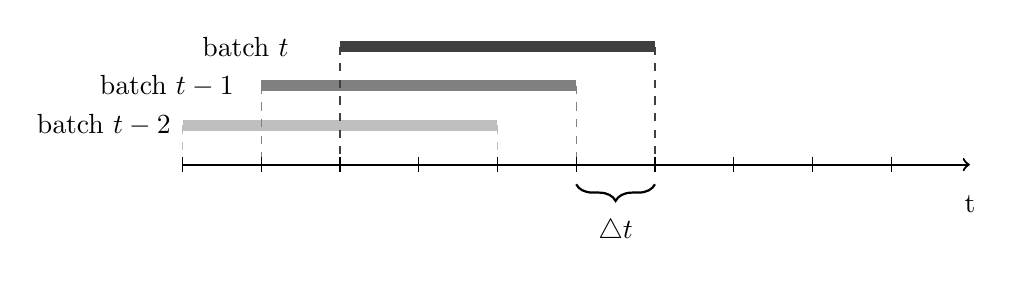
\begin{tikzpicture}[scale=1]

        \draw[lightgray, line width=4pt] (0,.5) -- (4,.5);
        \draw[lightgray, dashed] (0,.5) -- (0,0);
        \draw[lightgray, dashed] (4,.5) -- (4,0);
        \node[align=right] at (-1,.5) {batch $t - 2$};

        \draw[gray, line width=4pt] (1,1) -- (5,1);
        \draw[gray, dashed] (1,1) -- (1,0);
        \draw[gray, dashed] (5,1) -- (5,0);
        \node[align=right] at (-.2,1) {batch $t - 1$};

        \draw[darkgray, line width=4pt] (2,1.5) -- (6,1.5);
        \draw[darkgray, dashed] (2,1.5) -- (2,0);
        \draw[darkgray, dashed] (6,1.5) -- (6,0);
        \node[align=right] at (0.8,1.5) {batch $t$};

        \node[align=center] at (5.5,-0.85) {$\triangle t$};
        \node[align=center] at (10,-0.5) {t};

        \draw [thick,->] (0,0) -- (10,0);
        \foreach \x in {0,...,9} \draw (\x,0.1) -- (\x,-0.1);

        \draw [thick,decorate,decoration={brace,amplitude=6pt,raise=0pt,mirror}] (5,-0.25) -- (6,-0.25);

        \end{tikzpicture}

    \caption{Timeline showing the sliding window approach.}
    \label{fig:timeline}
\end{figure}

The overlap between batches depends on the batch size and the number of new samples in $\triangle t$.
A high volume of incoming samples combined with a small batch sizes
would result in an overlap too small to find pairs of clusters.
All clusters from the current batch would be detected as new in such a case.
To decrease the negative impact on the event detection by peaks in the data stream,
we need a batch size which grows accordingly.
The ideal batch size therefore provides enough overlap between batches to find pairs of clusters
and small enough to allow for efficient processing.
We explore three different methods for determining the ideal batch size:

\begin{enumerate}
    \item \textbf{Fixed size}: The first method uses a fixed batch size,
          where each batch processes the most recent \textit{n} samples.
          This makes the clustering unstable against sudden peaks in the volume of incoming data,
          but we consider this method as an useful benchmark for the dynamic methods.
    \item \textbf{Size by hours}: This method uses a dynamic batch size
          by loading the samples from the last \textit{n} hours.
          This enables the batch size to increase and decrease with the volume of the data stream.
          The number of samples will be limited by an upper bound,
          to keep the space and time consumption of the clustering method reasonable.
    \item \textbf{Size by incoming data}: This method defines the batch size relative to the incoming stream of data.
          We count the number of new samples since the last batch and multiply it by a predefined factor.
          For example if we want the new samples to be 1\%
          of the overall clustering, we define the factor as 100.
          The batch size will be limited by a lower and an upper bound.
          The lower bound prevents the overlap between batches from getting too small.
          The upper bound is based on the same reasoning as mentioned in the previous method.
\end{enumerate}

The evaluation will use the MP-Score to measure the precision of the event detection,
since our model represents events as a clusters.
True events can be extracted directly from the ground truth based on news articles from two successive batches.

\subsubsection{Implementation}
\label{subsubsec:4c_implementation}

The online clustering implemented for this thesis does not operate in a true online setting,
but rather it takes our existing test data and simulates a data stream over time.
The simulated approach allows us to directly compare the resulting events
with the ground truth and thus evaluate different settings.
The implementation is done with Python and runs in a dockerized environment similar to the evaluation framework.

The detection of events relies on comparing clusters between successive batches. 
We apply \gls{lsh}\cite{alex2015practical} to find clusters most similar to each other.
In its essence \gls{lsh} is an efficient way to find similar documents, 
which does not require to calculate the similarity between each possible pair of documents. 
The implementation for \gls{lsh} is provided by the datasketch library\cite{eric_zhu_2017_290602}.

Once we have found pairs of clusters, which represent the same story, detecting events becomes trivial.
For each pair we subtract the current cluster with the cluster from the previous batch. 
The resulting set contains all news articles, which are only present in the current cluster.
These articles are then summarized as a change of an existing event. 
If the previous batch did not contain any similar clusters for a cluster from the current batch, 
the cluster is considered as a new event.

Since events are themselves clusters of news articles,
we apply the MP-Score to measure the precision of detected events. 
Calculating the score is $O(n^2)$, but since the application runs on a simulated timeline and the scoring is only part of the evaluation,
time complexity is a minor concern in this case.

\paragraph{CLI}
The application provides a command line interface to run the simulation with different parameters
such as the start date, number of days to run and the batch size.

\begin{lstlisting}[caption=Command line interface for the online clustering., label={lst:cli_online_clustering}]
usage: online_clustering.py [-h] [--verbose] [--persist_in_db] 
                            [--rows ROWS] [--hours HOURS] 
                            [--factors FACTORS] --date DATE
                            [--run_n_days RUN_N_DAYS] 
                            [--threshold THRESHOLD]

Run the batchwise clustering over a simulated stream of news articles.

optional arguments:
-h, --help              show this help message and exit
--verbose               default: False
--persist_in_db         default: False
--rows ROWS             numbers of samples to process per batch
--hours HOURS           numbers of hours to load samples
--factors FACTORS       factor to use for relative batch sizes
--date DATE             start date
--run_n_days RUN_N_DAYS number of days to run the batchwise clustering
                        default: 1
--threshold THRESHOLD   similarity threshold for cluster matching
                        default: 0.75

\end{lstlisting}

